\documentclass[
	12pt,				% tamanho da fonte
	oneside,			% para impressão em recto e verso. Oposto a oneside
	a4paper,			% tamanho do papel. 
	english,			% idioma adicional para hifenização
	brazil,				% o último idioma é o principal do documento
	]{abntex2}

% ---
% Pacotes fundamentais 
% ---
\usepackage{lmodern}			% Usa a fonte Latin Modern
\usepackage[T1]{fontenc}		% Selecao de codigos de fonte.
\usepackage[utf8]{inputenc}		% Codificacao do documento (conversão automática dos acentos)
\usepackage{indentfirst}		% Indenta o primeiro parágrafo de cada seção.
\usepackage{color}				% Controle das cores
\usepackage{graphicx}			% Inclusão de gráficos
\usepackage{microtype} 			% para melhorias de justificação
\usepackage{multicol}
\usepackage{multirow}
\usepackage[brazilian,hyperpageref]{backref}	 % Paginas com as citações na bibl
\usepackage[alf]{abntex2cite}	% Citações padrão ABNT
\usepackage{listings}
\usepackage{float}

\lstset{
  showspaces=false,
  showtabs=false,
  breaklines=true,
  showstringspaces=false,
  breakatwhitespace=true,
  commentstyle=\color{green},
  keywordstyle=\color{blue},
  stringstyle=\color{red},
  basicstyle=\ttfamily
}

% --- 
% CONFIGURAÇÕES DE PACOTES
% --- 

% ---
% Configurações do pacote backref
% Usado sem a opção hyperpageref de backref
\renewcommand{\backrefpagesname}{Citado na(s) página(s):~}
% Texto padrão antes do número das páginas
\renewcommand{\backref}{}
% Define os textos da citação
\renewcommand*{\backrefalt}[4]{
	\ifcase #1 %
		Nenhuma citação no texto.%
	\or
		Citado na página #2.%
	\else
		Citado #1 vezes nas páginas #2.%
	\fi}%
% ---

% ---
% Informações de dados para CAPA e FOLHA DE ROSTO
% ---
\titulo{Prática 9: Regex}
\autor{Pedro Inácio Rodrigues Pontes}
\local{Belo Horizonte, Brasil}
\data{2025}
\instituicao{%
  Universidade Federal de Minas Gerais
  \par
  Colégio Técnico
  \par
  Curso Técnico em Desenvolvimento de Sistemas}

\definecolor{blue}{RGB}{41,5,195}

\makeatletter
\hypersetup{
     	%pagebackref=true,
		pdftitle={\@title}, 
		pdfauthor={\@author},
    	pdfsubject={\imprimirpreambulo},
		colorlinks=true,       		% false: boxed links; true: colored links
    	linkcolor=blue,          	% color of internal links
    	citecolor=blue,        		% color of links to bibliography
    	filecolor=magenta,      		% color of file links
		urlcolor=blue,
		bookmarksdepth=4
}
\makeatother

\renewcommand{\thesection}{\arabic{section}}
\setlength{\parindent}{1.3cm}
\setlength{\parskip}{0.2cm} 

\makeindex


\begin{document}

\selectlanguage{brazil}
\frenchspacing 

\imprimircapa

{
\ABNTEXchapterfont

\textual

% ----------------------------------------------------------
% Introdução (exemplo de capítulo sem numeração, mas presente no Sumário)
% ----------------------------------------------------------
\section{Introdução}

O objetivo deste projeto é desenvolver duas aplicações distintas em C\# que demonstrem conceitos fundamentais de Regex. A primeira aplicação consiste em um programa de console que implementa um sistema de validação de senhas com critérios de segurança rigorosos, solicitando ao usuário a digitação repetida de senhas até que uma senha considerada "forte" seja fornecida. O sistema deve verificar se a senha inserida atende aos seguintes requisitos: possuir entre 7 e 16 caracteres, conter pelo menos uma letra minúscula (a-z), uma letra maiúscula (A-Z), um dígito (0-9) e um caractere especial dentre os seguintes símbolos:

\begin{lstlisting}
! @ # $ % ^ & * ( ) + = _ - { } [ ] : ; " ' ? < > , .
\end{lstlisting}

Para essa validação, será utilizada a expressão regular:

\begin{lstlisting}
@"^(?=.*[a-z])(?=.*[A-Z])(?=.*\d)
(?=.*[!@#$%^&*()+=_\-{}\[\]:;""'?<>,.]).{7,16}$"
\end{lstlisting}

cujo funcionamento e estrutura serão detalhadamente explicados. A segunda aplicação envolve o processamento de dados em formato JSON contendo informações sobre os Prêmios Nobel, com foco específico na extração e listagem dos primeiros nomes (firstname) dos ganhadores do prêmio de economia (categoria "economics"). Ambas as aplicações demonstram práticas essenciais de desenvolvimento em C#, incluindo validação de entrada de dados, uso de expressões regulares, manipulação de arquivos JSON e tratamento adequado de erros, proporcionando uma base sólida para o entendimento de conceitos fundamentais de programação orientada a objetos e processamento de dados estruturados.

\section{Desenvolvimento}

\subsection{Validação de Senhas}

O programa de validação de senhas implementa um sistema que utiliza uma expressão regular para verificar critérios de segurança rigorosos, executando um loop contínuo que solicita senhas ao usuário até que uma senha considerada forte seja fornecida. O código utiliza a biblioteca System.Text.RegularExpressions e define uma variável estática para armazenar a senha digitada pelo usuário.

\begin{lstlisting}[language=C]
using System.Text.RegularExpressions;
class Program
{
    static string? Password;
    public static void Main(string[] args)
    {
        string regexPattern = @"^(?=.*[a-z])(?=.*[A-Z])(?=.*\d)
        (?=.*[!@#$%^&*()+=_\-{}\[\]:;""'?<>,.]).{7,16}$";
        while (true)
        {
            Console.WriteLine("Digite a senha a ser verificada:");
            Password = Console.ReadLine();
            if (Regex.IsMatch(Password, regexPattern))
            {
                Console.WriteLine("Senha forte!");
                return;
            }
            Console.WriteLine("Senha fraca, tente novamente");
        }
    }
}
\end{lstlisting}

A expressão regular utilizada é composta por várias partes que trabalham em conjunto para garantir todos os critérios de segurança estabelecidos. O símbolo circunflexo no início da expressão indica o começo da string, enquanto o símbolo de cifrão ao final indica o término, garantindo que toda a string seja validada do início ao fim. Os lookaheads positivos, representados pela sintaxe (?=...), são elementos fundamentais que verificam condições específicas sem consumir caracteres da string, permitindo que múltiplas validações sejam aplicadas simultaneamente sobre a mesma entrada. O primeiro lookahead (?=.*[a-z]) verifica se existe pelo menos uma letra minúscula em qualquer posição da string, seguido por (?=.*[A-Z]) que confirma a presença de pelo menos uma letra maiúscula. O terceiro lookahead \verb|(?=.*\d)| assegura que há pelo menos um dígito numérico, enquanto o quarto lookahead verifica a existência de pelo menos um caractere especial da lista definida entre os colchetes. Por fim, a expressão \verb|.{7,16}| corresponde a qualquer caractere repetido entre 7 e 16 vezes, definindo assim o comprimento mínimo e máximo aceitável para a senha. Este mecanismo de lookaheads é essencial pois permite que todos os critérios sejam verificados independentemente da ordem em que os caracteres aparecem na senha digitada pelo usuário.

\subsection{Nome dos Vencendores do Nobel de Economia}

A segunda aplicação desenvolvida realiza o processamento de dados JSON contendo informações sobre os Prêmios Nobel, com o objetivo específico de extrair os primeiros nomes dos ganhadores do prêmio de economia. O programa utiliza técnicas avançadas de manipulação de strings através de expressões regulares para analisar a estrutura hierárquica do arquivo JSON e localizar informações específicas dentro de categorias determinadas.

\begin{lstlisting}[language=C]
using System.Text.RegularExpressions;
string json = File.ReadAllText("prize.json");
string pattern = @"""category"":""economics"".*?""laureates"":\s*\[(.*?)\]";
MatchCollection matches = Regex.Matches(json, pattern);
List<string> names = new List<string>();
foreach (Match match in matches)
{
    string contentLaureates = match.Groups[1].Value;
    string namePattern = @"""firstname"":""([^""]+)""";
    MatchCollection namesMatches = Regex.Matches(contentLaureates, namePattern);
    foreach (Match nameMatch in namesMatches)
    {
        string name = nameMatch.Groups[1].Value;
        names.Add(name);
    }
}
Console.WriteLine("Ganhadores do Nobel de Economia:");
foreach (string name in names)
{
    Console.WriteLine(name);
}
\end{lstlisting}

O programa inicia carregando todo o conteúdo do arquivo prize.json na memória através do método File.ReadAllText. A primeira expressão regular utilizada busca especificamente por seções do JSON que contenham a categoria "economics", utilizando o padrão que localiza a palavra "category" seguida de "economics" e posteriormente captura todo o conteúdo da seção "laureates" correspondente. A expressão utiliza grupos de captura, onde a sintaxe (.*?) dentro dos parênteses captura de forma não-gulosa todo o conteúdo entre os colchetes que definem o array de laureados. Para cada correspondência encontrada, o programa extrai o conteúdo capturado pelo primeiro grupo e aplica uma segunda expressão regular específica para localizar os primeiros nomes. O padrão utilizado para extrair os nomes busca pela chave "firstname" seguida de dois pontos e aspas, capturando qualquer sequência de caracteres que não sejam aspas através da classe de caracteres negativa \verb|[^"]|. Esta abordagem garante que apenas o valor do primeiro nome seja extraído, excluindo as aspas delimitadoras. O programa utiliza uma estrutura de dados List para armazenar todos os nomes encontrados e posteriormente os exibe no console de forma organizada, precedidos por um cabeçalho identificativo.

\section{Resultados}

\begin{figure}[H]
    \centering
    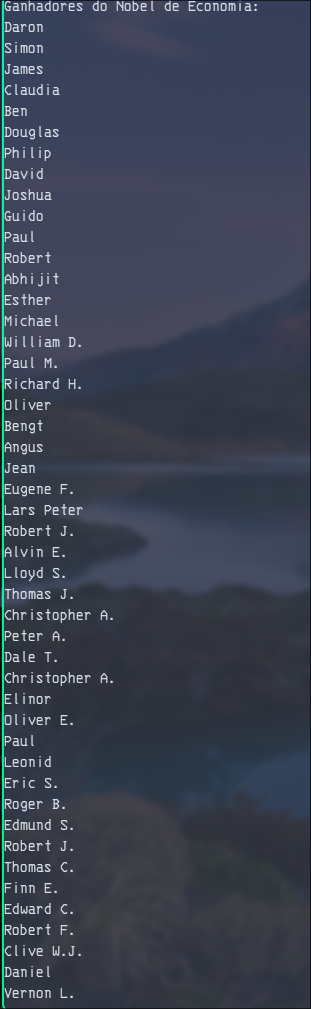
\includegraphics[width=1\textwidth]{imgs/img1.png}
    \label{fig:img1}
\end{figure}

\begin{figure}[H]
    \centering
    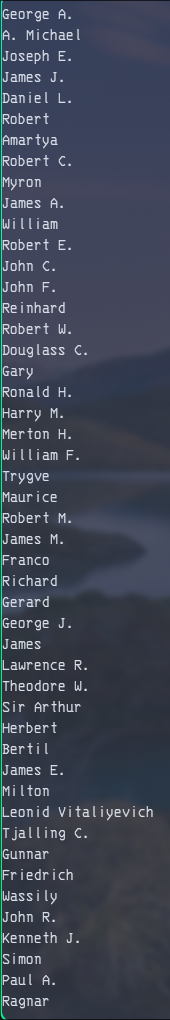
\includegraphics[width=1\textwidth]{imgs/img2.png}
    \label{fig:img2}
\end{figure}

\begin{figure}[H]
    \centering
    
\includegraphics[width=1\textwidth]{imgs/img3.png}
    \caption{Vencedores do Nobel de Economia}
    \label{fig:img3}
\end{figure}

\begin{figure}[H]
    \centering
    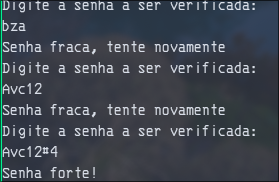
\includegraphics[width=1\textwidth]{imgs/img4.png}
    \caption{Verificação de Senhas}
    \label{fig:img4}
\end{figure}

\section{Conclusão}

O desenvolvimento das duas aplicações em C# demonstrou a eficácia das expressões regulares na validação de dados e no processamento de informações estruturadas. O programa de validação de senhas implementou com sucesso critérios rigorosos de segurança através de lookaheads positivos, garantindo que todas as condições sejam verificadas simultaneamente. A aplicação de processamento JSON mostrou como expressões regulares podem ser utilizadas para extrair dados específicos de arquivos estruturados, permitindo a localização e captura precisa dos primeiros nomes dos ganhadores do Nobel de Economia. Ambos os projetos evidenciaram a importância do tratamento adequado de strings e da aplicação de técnicas de programação robustas para manipulação de dados, consolidando conhecimentos fundamentais sobre processamento de arquivos e uso de expressões regulares em aplicações práticas de console.

\end{document}
